\documentclass[11pt]{amsart}

\renewcommand{\baselinestretch}{1.08}

\usepackage{geometry}
\geometry{letterpaper, margin=1in}

\usepackage{verbatim,xspace,amssymb}

\usepackage{tikz}
\usetikzlibrary{arrows}

% math macros
\newcommand\bb{\mathbf{b}}
\newcommand\bbf{\mathbf{f}}
\newcommand\bn{\mathbf{n}}
\newcommand\bq{\mathbf{q}}
\newcommand\bu{\mathbf{u}}
\newcommand\bv{\mathbf{v}}
\newcommand\by{\mathbf{y}}

\newcommand\bQ{\mathbf{Q}}
\newcommand\bV{\mathbf{V}}
\newcommand\bX{\mathbf{X}}

\newcommand\CC{\mathbb{C}}
\newcommand{\DDt}[1]{\ensuremath{\frac{d #1}{d t}}}
\newcommand{\ddt}[1]{\ensuremath{\frac{\partial #1}{\partial t}}}
\newcommand{\ddx}[1]{\ensuremath{\frac{\partial #1}{\partial x}}}
\newcommand{\ddy}[1]{\ensuremath{\frac{\partial #1}{\partial y}}}
\newcommand{\ddxp}[1]{\ensuremath{\frac{\partial #1}{\partial x'}}}
\newcommand{\ddz}[1]{\ensuremath{\frac{\partial #1}{\partial z}}}
\newcommand{\ddxx}[1]{\ensuremath{\frac{\partial^2 #1}{\partial x^2}}}
\newcommand{\ddyy}[1]{\ensuremath{\frac{\partial^2 #1}{\partial y^2}}}
\newcommand{\ddxy}[1]{\ensuremath{\frac{\partial^2 #1}{\partial x \partial y}}}
\newcommand{\ddzz}[1]{\ensuremath{\frac{\partial^2 #1}{\partial z^2}}}
\newcommand{\Div}{\nabla\cdot}
\newcommand\eps{\epsilon}
\newcommand{\grad}{\nabla}
\newcommand{\ihat}{\mathbf{i}}
\newcommand{\ip}[2]{\ensuremath{\left<#1,#2\right>}}
\newcommand{\jhat}{\mathbf{j}}
\newcommand{\khat}{\mathbf{k}}
\newcommand{\nhat}{\mathbf{n}}
\newcommand\lam{\lambda}
\newcommand\lap{\triangle}
\newcommand\Matlab{\textsc{Matlab}\xspace}
\newcommand\RR{\mathbb{R}}
\newcommand\vf{\varphi}

\newcommand{\Mstar}{$\text{Mahaffy}^\star$\xspace}

\newcommand\alpharight{\alpha_{{}_{\blacktriangleright}}}
\newcommand\alphaup{\alpha_{{\!}_{\blacktriangle}}}

\newcommand{\dxtwo}{\tfrac{\Delta x}{2}}
\newcommand{\dytwo}{\tfrac{\Delta y}{2}}



\title[The Mahaffy scheme is a finite element method]{The Mahaffy (1976) numerical scheme for the \\ shallow ice approximation is a finite element method}

\author{Ed Bueler}


\begin{document}

%\begin{abstract}
%\end{abstract}

\maketitle

\thispagestyle{empty}


\section{Introduction}

The finite difference (FD) scheme introduced by \cite{Mahaffy1976} for modeling the Barnes Ice Cap was used in the first clear success in modeling ice sheet flow and geometry evolution in two horizontal dimensions.  This scheme is a widely-used choice for numerically solving the shallow ice approximation, and its accuracy properties are relatively-well understood \cite{Bueleretal2005}.   The scheme computes the ice flux at staggered-grid points using particular choices when evaluating the ice surface slope and thickness.  In a test where an analytical solution is known and the ice rheology is realistic, these choices imply higher accuracy than an alternative widely-used scheme, while using a smaller stencil (``computational molecule''), thereby reducing memory usage in implicit implementations \cite{HindmarshPayne1996}.  As a scheme for non-sliding glacier flow, it is used as part of the stress balance solution method in a membrane-stress-resolving hybrid ice dynamics model \cite{BuelerBrown2009}.

We show that in the structured grid case the Mahaffy scheme is a reasonable, though not standard, quadrature choice for a conforming Petrov-Galerkin finite element (FE) method \cite{Elmanetal2005}.  The trial functions are piecewise-bilinear on a structured grid of rectangles---i.e.~$Q^1$ finite elements \cite{Elmanetal2005}.  The test functions are piecewise-constant with support on dual rectangular control volumes, so the scheme can also be interpreted as a ``finite volume element'' (FVE) method \cite{EwingLinLin2002}.

PROPOSE: Based on this re-interpretation of the scheme we propose, and test, a ``\Mstar'' scheme which uses a more accurate quadrature choice when evaluating the relevant flux integral, but based on the same stencil.  PROPOSE: Furthermore, we can construct this \Mstar scheme on unstructured grids consisting of suitable finite element triangulations with dual control volumes, i.e.~Delaunay/Voronoi dual meshes (compare \cite{Ringleretal2013}).

MAYBE NOT: The accuracy of the Mahaffy scheme on steep bed terrain has been found to be flawed, but corrections have been proposed \cite{JaroschSchoofAnslow2013}.  We show that these corrections are unnecessary in the \Mstar scheme.


\section{The Mahaffy finite difference scheme}  The shallow ice approximation (SIA) \cite{Hutter1983} is the lubrication approximation \cite{Fowler1997} of the Stokes equations for slow-flowing ice which is in non-sliding contact with the bed and which has a freely-evolving upper surface.  We only consider the isothermal, Glen-power-law (e.g.~\cite{GreveBlatter2009}) case of the shallow ice approximation.

Let $H$ be the ice thickness, $b$ the bed elevation, and $s = H+b$ the ice surface elevation.  The ice sheet thickness evolution itself is a straightforward conservation equation,
\begin{equation}
\frac{\partial H}{\partial t} + \Div \bq = m  \label{eq:siaevolution}
\end{equation}
where $m$ [SI units $\text{m}/\text{s}$] is the surface mass balance, also called the accumulation/ablation function, and the divergence ``$\Div$'' is computed in horizontal $x,y$ directions only.  In the SIA the vertically-integrated flux [units $\text{m}^2/\text{s}$], or volume flux \cite{GreveBlatter2009}, is
\begin{equation}
\bq = - \Gamma H^{n+2} |\grad s|^{n-1} \grad s  \label{eq:siaflux}
\end{equation}
where $\Gamma = 2 A (\rho g)^n / (n+2)$ is a positive constant, in the isothermal case, and ``$\grad$'' is the gradient in $x,y$.

The flux \eqref{eq:siaflux} has a couple of interpretations in the literature.  Equation \eqref{eq:siaevolution} can be interpreted as a nonlinear diffusion equation with a flux
\begin{equation}
\bq = - D \grad s, \quad \text{where} \quad D =  \Gamma H^{n+2} |\grad s|^{n-1}. \label{eq:siafluxdiffusion}
\end{equation}
On the other hand, one can compute a vertically-averaged velocity, and define the flux that way,
\begin{equation}
\bq = \bar \bv H, \quad \text{where} \quad \bar \bv = - \Gamma H^{n+1} |\grad s|^{n-1} \grad s, \label{eq:siafluxvelocity}
\end{equation}
in which case \eqref{eq:siaevolution} is a superficially-hyperbolic conservation equation.  However, the former diffusion interpretation is surely more appropriate in the flat-bed case $b=0$, as \eqref{eq:siaevolution} can be transformed to a $p$-Laplacian diffusion equation \cite{CDDSV} in that case, but in general the diffusion-equation interpretation of \eqref{eq:siaevolution} is obscured by the bed gradient $\grad b$ appearing implicitly in formula \eqref{eq:siafluxdiffusion} for $D$ \cite{JouvetBueler2012}.

Because our interest is only in spatial discretization aspects, from now on we only consider the steady-state case of \eqref{eq:siaevolution}, namely
\begin{equation}
\Div \bq = m,  \label{eq:siasteady}
\end{equation}
solved in some domain $\Omega$ in the plane.  The input data to \eqref{eq:siasteady} consists of the bed elevation $b(x,y)$ and the (steady) surface mass balance $m(x,y)$ defined on $\Omega$.  The solution is the nonnegative thickness function $H(x,y)$, which gives the corresponding surface elevation $s(x,y)$.  If the $m$ is sufficiently-negative near the boundary of $\Omega$ then $H$ reaches zero inside the domain at a free boundary \cite{JouvetBueler2012}.  This free boundary, at which both $H\to 0$ and $\bq \to 0$, also has degenerate diffusivity $D \to 0$.  Solving \eqref{eq:siasteady} as such a free-boundary problem, or solving each step of a time-stepping method for \eqref{eq:siaevolution} as a free-boundary problem, is usually called a ``whole ice sheet'' model.

The Mahaffy scheme calculates the vertically-integrated ice flux $\bq$ at the staggered grid points \cite[equations (19), (20)]{Mahaffy1976}.  Consider the FD grid in Figure \ref{fig:fdfemgrids}a.  At the staggered location $(x_{j+1/2},y_k)$, the scheme computes the $x$-component of the flux by
\begin{equation}
q^x_{j+1/2,k} = - \Gamma \left(\tfrac{H_{j,k} + H_{j+1,k}}{2}\right)^{n+2} \alpharight^{\,n-1} \tfrac{s_{j+1,k} - s_{j,k}}{\Delta x}  \label{eq:mahaffyWqx}
\end{equation}
where $s_{j,k} = H_{j,k} + b_{j,k}$.  The quantity ``$\alpharight$\!'' is an estimate of the surface slope $|\grad s|$, a key quantity in \eqref{eq:siaflux}, at the staggered-grid location:
\begin{equation}
\alpharight^{\,2} = \left(\tfrac{s_{j+1,k} - s_{j,k}}{\Delta x}\right)^2 + \left(\tfrac{s_{j,k+1} + s_{j+1,k+1} - s_{j,k-1} - s_{j+1,k-1}}{4 \Delta y}\right)^2.  \label{eq:mahaffyWalphax}
\end{equation}
The formula for the flux $q^y_{j,k+1/2}$ at the staggered-grid location $(x_j,y_{k+1/2})$, at the center of the top edge of the control volume, follow by swapping the roles of $j$ and $k$ in equations \eqref{eq:mahaffyWqx} and \eqref{eq:mahaffyWalphax}:
\begin{align}
q^y_{j,k+1/2} &= - \Gamma \left(\tfrac{H_{j,k} + H_{j,k+1}}{2}\right)^{n+2} \alphaup^{\,n-1} \tfrac{s_{j,k+1} - s_{j,k}}{\Delta y}, \label{eq:mahaffyWqy} \\
\alphaup^{\,2} &= \left(\tfrac{s_{j+1,k} + s_{j+1,k+1} - s_{j-1,k} - s_{j-1,k+1}}{4 \Delta x}\right)^2 + \left(\tfrac{s_{j,k+1} - s_{j,k}}{\Delta y}\right)^2.  \label{eq:mahaffyWalphay}
\end{align}
Slope approximations \eqref{eq:mahaffyWalphax} and \eqref{eq:mahaffyWalphay} are perhaps the least-obvious aspect of the Mahaffy scheme.  Solving SIA equation \eqref{eq:siasteady} then uses straightforward centered-difference formulas \cite{MortonMayers2005} for the flux divergence:
\begin{equation}
\frac{q^x_{j+1/2,k} - q^x_{j-1/2,k}}{\Delta x} + \frac{q^y_{j,k+1/2}- q^y_{j,k-1/2}}{\Delta y} = m_{j,k}.  \label{eq:siasteadyfd}
\end{equation}

\begin{figure}[ht]
\begin{center}
\begin{tikzpicture}[scale=0.75]
  %uncomment to see grid on which it was generated:
  %\draw[dotted,step=1.0,black,very thin] (0,0) grid (6,4);

  % faint grid
  \draw[gray, dashed] (-0.75,0) -- (6.75,0);
  \draw[gray, dashed] (-0.75,2) -- (6.75,2);
  \draw[gray, dashed] (-0.75,4) -- (6.75,4);
  \draw[gray, dashed] (0,-0.5) -- (0,4.5);
  \draw[gray, dashed] (3,-0.5) -- (3,4.5);
  \draw[gray, dashed] (6,-0.5) -- (6,4.5);

  % regular FD points
  \filldraw (0,0) circle (2.5pt);
  \filldraw (3,0) circle (2.5pt);
  \filldraw (6,0) circle (2.5pt);
  \filldraw (0,2) circle (2.5pt);
  \filldraw (3,2) circle (2.5pt);
  \filldraw (6,2) circle (2.5pt);
  \filldraw (0,4) circle (2.5pt);
  \filldraw (3,4) circle (2.5pt);
  \filldraw (6,4) circle (2.5pt);

  % staggered FD points
  \def\dx{0.12};
  \filldraw (1.5-\dx,2+\dx) -- (1.5+\dx,2) -- (1.5-\dx,2-\dx) -- cycle;
  \filldraw (4.5-\dx,2+\dx) -- (4.5+\dx,2) -- (4.5-\dx,2-\dx) -- cycle;
  \filldraw (3-\dx,1-\dx) -- (3,1+\dx) -- (3+\dx,1-\dx) -- cycle;
  \filldraw (3-\dx,3-\dx) -- (3,3+\dx) -- (3+\dx,3-\dx) -- cycle;

  % dimensions \Delta x, \Delta y
  \draw[latex-latex] (3.2,4.5) -- (5.8,4.5);
  \draw (4.5,5.0) node {$\Delta x$};
  \draw[latex-latex] (6.5,2.2) -- (6.5,3.8);
  \draw (7.0,3) node {$\Delta y$};

  % label center point and dims
  \draw (3,-1.0) node {$x_j$};
  \draw (-1.25,2) node {$y_k$};

  % label as "a"
  \draw (-1.5,5.5) node {{\large a.}};
\end{tikzpicture}
 \quad 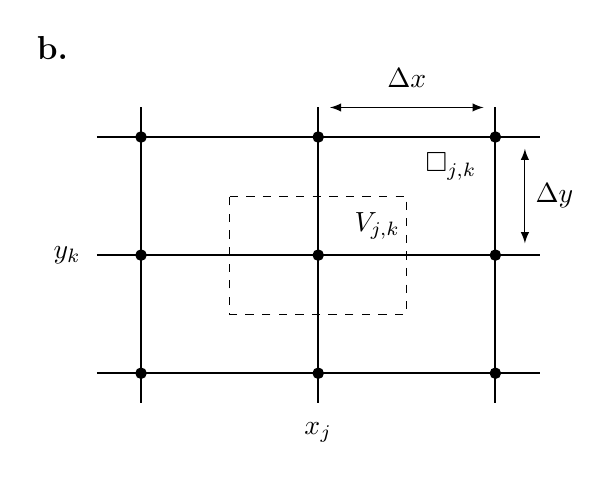
\begin{tikzpicture}[scale=0.75]
  %uncomment to see grid on which it was generated:
  %\draw[dotted,step=1.0,black,very thin] (0,0) grid (6,4);

  % strong grid around elements
  \draw[thick] (-0.75,0) -- (6.75,0);
  \draw[thick] (-0.75,2) -- (6.75,2);
  \draw[thick] (-0.75,4) -- (6.75,4);
  \draw[thick] (0,-0.5) -- (0,4.5);
  \draw[thick] (3,-0.5) -- (3,4.5);
  \draw[thick] (6,-0.5) -- (6,4.5);

  % nodes
  \filldraw (0,0) circle (2.5pt);
  \filldraw (3,0) circle (2.5pt);
  \filldraw (6,0) circle (2.5pt);
  \filldraw (0,2) circle (2.5pt);
  \filldraw (3,2) circle (2.5pt);
  \filldraw (6,2) circle (2.5pt);
  \filldraw (0,4) circle (2.5pt);
  \filldraw (3,4) circle (2.5pt);
  \filldraw (6,4) circle (2.5pt);

  % outline control volume
  \draw[dashed] (1.5,3) -- (4.5,3) -- (4.5,1) -- (1.5,1) -- cycle;

  % label element and control volume
  \draw (5.25,3.5) node {$\square_{j,k}$};
  \draw (4,2.5) node {$V_{j,k}$};

  % dimensions \Delta x, \Delta y
  \draw[latex-latex] (3.2,4.5) -- (5.8,4.5);
  \draw (4.5,5.0) node {$\Delta x$};
  \draw[latex-latex] (6.5,2.2) -- (6.5,3.8);
  \draw (7.0,3) node {$\Delta y$};

  % label center point and dims
  \draw (3,-1.0) node {$x_j$};
  \draw (-1.25,2) node {$y_k$};

  % label as "b"
  \tikzstyle{fontbf} = [font=\bf]
  \draw (-1.5,5.5) node[fontbf] {{\large b.}};
\end{tikzpicture}

\end{center}
\caption{Left: A structured FD grid with regular (dots) and staggered (triangles) grid locations.  Right: A structured FE grid with rectangular elements (solid), degrees of freedom at the nodes (dots), and dual rectangular control volumes (dashed).}
\label{fig:fdfemgrids}
\end{figure}


\section{A finite element interpretation}

The above description of the Mahaffy FD method is familiar to numerical ice sheet modelers, but deriving the same scheme from a FE perspective, as we do now, is new.  This re-interpretation uses the same structured grid, but the regular grid points $(x_j,y_k)$ are now nodes (i.e.~degrees of freedom) for a continuous and piecewise-bilinear space of trial functions.  The nodes are also used as centered degrees of freedom for piecewise-constant test functions which are discontinuous at the same locations as the FD method's staggered grid points.  The method is of ``Petrov-Galerkin'' type because the trial and test functions come from different spaces \cite{Elmanetal2005}, but our choice make it a ``finite volume element'' (FVE) method \cite{EwingLinLin2002} also.  Exact discrete conservation follows in the standard finite volume (FV) understanding \cite{LeVeque}.

Consider the structured grid of rectangles with dimensions $\Delta x,\Delta y$ shown in Figure \ref{fig:fdfemgrids}b.  The rectangle $\square_{j,k}$ has lower-left corner at $(x_j,y_k)$.  These rectangles are $Q^1$ finite elements when associated with bilinear functions.  A basis of bilinear functions on $\square_{j,k}$ is
\begin{equation}
\chi_l(x-x_j,y-y_k), \label{eq:elementbasis}
\end{equation}
for $l=1,2,3,4$, where
\begin{align*}
\chi_1(x,y) &= \left(1-\tfrac{x}{\Delta x}\right) \left(1-\tfrac{y}{\Delta y}\right), & \chi_2(x,y) &= \tfrac{x}{\Delta x} \left(1-\tfrac{y}{\Delta y}\right), \\
\chi_3(x,y) &= \left(1-\tfrac{x}{\Delta x}\right) \tfrac{y}{\Delta y}, & \chi_4(x,y) &= \tfrac{x}{\Delta x} \tfrac{y}{\Delta y}. 
\end{align*}
If $C(\Omega)$ denotes the continuous functions on the domain, then let
\begin{equation}
S_h = \{u \in C(\Omega) \,\big|\, u \text{ is bilinear on each $\square_{j,k}$}\},
\end{equation}
the $Q^1$ finite element space \cite{Elmanetal2005}.  Functions in $S_h$ have a gradient which is defined almost everywhere, but the gradient is discontinuous along the element edges (i.e.~along solid lines in Figure \ref{fig:fdfemgrids}b).

Let $V_{j,k}$ be the rectangular control volume shown by dashed lines in Figure \ref{fig:fdfemgrids}b, with center at $(x_j,y_j)$.  If $L^\infty(\Omega)$ denotes bounded and integrable functions on $\Omega$, then let
\begin{equation}
S_h^* = \{u \in L^\infty(\Omega) \,\big|\, u \text{ is constant on each $V_{j,k}$}\}.
\end{equation}
Functions in $S_h^*$ are discontinuous along the control volume edges (dashed lines in Figure \ref{fig:fdfemgrids}b).

If the nodes $(x_j,y_k)$ have index $j$ in $1,\dots,N_x$ and index $k$ in $1,\dots,N_y$, so there are $N_xN_y$ distinct nodes, then $\dim S_h = \dim S_h^* = N_x N_y$.  Bases of $S_h$ and $S_h^*$ are easy to give, by choosing functions which take value one at a single node and are zero at all other nodes.  By definition, $\psi_{j,k}$ is the unique function in $S_h$ so that $\psi_{j,k}(x_r,y_s) = \delta_{jr} \delta_{ks}$, and $\omega_{j,k}$ is the unique function in $S_h^*$  so that $\omega_{j,k}(x_r,y_s) = \delta_{jr} \delta_{ks}$.  See Figure \ref{fig:fembases}.

\begin{figure}[ht]
\begin{center}
FIXME
%\includegraphics[width=2.0in,keepaspectratio=true]{FIXME}
\end{center}
\caption{Left: A ``hat'' basis function $\psi_{j,k}(x,y)$ in the trial space $S_h$.  Right: A piece-wise constant basis function $\omega_{j,k}(x,y)$ in the test space $S_h^*$.}
\label{fig:fembases}
\end{figure}

If \eqref{eq:siasteady} holds then multiplication by an integrable function $g(x,y)$, and integration, implies that
\begin{equation}
  \int_\Omega (\Div \bq)\, g\,dx\,dy = \int_\Omega m g\,dx\,dy.  \label{eq:siaweak}
\end{equation}
(Note we have not used the divergence theorem, i.e.~integration-by-parts, as in a ``Galerkin'' FEM method \cite{Elmanetal2005}.)  In our FE method, we seek an approximate solution $H^h$ from $S_h$.  Let $b^h$ be the piecewise-bilinear interpolant of the bed elevation $b(x,y)$ and let $s^h=H^h+b^h$.  We denote by $\bq^h$ the flux computed from formula \eqref{eq:siaflux} using $H^h$ and $b^h$.  Our idea is to require \eqref{eq:siaweak} to hold for this $\bq^h$ and for all $g$ in $S_h^*$.  However, it will suffice to only test for a basis of $S_h^*$, so $g=\omega_{j,k}$.  Also, because $\omega_{j,k}$ is equal to one on $V_{j,k}$ and is zero otherwise, we can use the divergence theorem just on $V_{j,k}$.  Finally, we can use midpoint quadrature on the right-hand integral.  Thus we seek $H^h$ in $S_h$ satisfying
\begin{equation}
  - \int_{\partial V_{j,k}} \bq^h \cdot \bn\,ds = m_{j,k}\, \Delta x \Delta y, \label{eq:siafve}
\end{equation}
for all $j,k$, where $\bn$ is the outward normal unit vector and $ds$ the length element on the closed curve (rectangle) $\partial V_{j,k}$.  Equation \eqref{eq:siafve} is actually a typical FV interpretation of equation \eqref{eq:siasteady}, but the FE character remains here because $\bq^h$ is defined almost everywhere on $\Omega$, as $H^h$ and $s^h$ are from a continuous function space $S_h$.

The FE method is completed by computing the integral in \eqref{eq:siafve}.  Though $\bq^h$ is a well-defined, bounded function, and continuous on each element $\square_{j,k}$, it is discontinuous across element boundaries.  We decompose the integral in \eqref{eq:siafve} into the four edges which form $\partial V_{j,k}$.  For this purpose let $x_j^\pm = x_j \pm \dxtwo$, $y_k^\pm = y_k \pm \dytwo$, and denote components $\bq^h = \ip{q^x}{q^y}$, so that
\begin{equation}
  \int_{\partial V_{j,k}} \bq^h \cdot \bn\,ds = \int_{y_k^-}^{y_k^+} q^x(x_j^+,y)\,dy + \int_{x_j^-}^{x_j^+} q^y(x,y_k^+)\,dx - \int_{y_k^-}^{y_k^+} q^x(x_j^-,y)\,dy - \int_{x_j^-}^{x_j^+} q^y(x,y_k^-)\,dx. \label{eq:fluxintdecomp}
\end{equation}
Note $q^x$ and $q^y$ are scalar functions that depend on $(x,y)$ through $H^h$ and $b^h$.

Considering the first of the integrals on the right in \eqref{eq:fluxintdecomp}, the integrand $f(y) = q^x(x_j^+,y)$ is piecewise-continuous on the interval of integration $y_k^- \le y \le y_k^+$.  It has a jump discontinuity at the midpoint $y=y_k$ because, though $\grad s^h = \ip{s^h_x}{s^h_y}$ is linear on each element, $s^h_y$ is discontinuous at $y=y_k$.  The Mahaffy scheme computes the integral by the midpoint method, but using $s^h_y$ \emph{averaged across its jump discontinuity} there, as though that average were a value.

To turn this idea into formulas, first note that the thickness $H^h$ and the $x$-derivative $s^h_x$ have continuous values between the elements $\square_{j,k}$ and $\square_{j,k-1}$.  In particular, writing-out $H^h(x,y)$ on either element, using the element basis \eqref{eq:elementbasis}, gives
\begin{equation}
H^h(x_j^+,y_k) = \tfrac{H_{j,k}+H_{j+1,k}}{2}, \label{eq:femHstag}
\end{equation}
Next, the components of the surface gradient on the element $\square_{j,k}$ have the formulas
	\begin{comment}
	COMMENT OUT: here is the surface elevation on $\square_{j,k}$
	\begin{align*}
	s^h(x,y) &= s_{j,k} \left(1-\tfrac{x-x_j}{\Delta x}\right) \left(1-\tfrac{y-y_k}{\Delta y}\right)
	    + s_{j+1,k} \left(\tfrac{x-x_j}{\Delta x}\right) \left(1-\tfrac{y-y_k}{\Delta y}\right) \\
	         &\qquad + s_{j,k+1} \left(1-\tfrac{x-x_j}{\Delta x}\right) \left(\tfrac{y-y_k}{\Delta y}\right)
	    + s_{j+1,k+1} \left(\tfrac{x-x_j}{\Delta x}\right) \left(\tfrac{y-y_k}{\Delta y}\right)
	\end{align*}
	\end{comment}
\begin{align}
s^h_x(x,y) &= \tfrac{s_{j+1,k}-s_{j,k}}{\Delta x} \left(1-\tfrac{y-y_k}{\Delta y}\right) + \tfrac{s_{j+1,k+1}-s_{j,k+1}}{\Delta x} \left(\tfrac{y-y_k}{\Delta y}\right), \label{eq:grads} \\
s^h_y(x,y) &= \tfrac{s_{j,k+1}-s_{j,k}}{\Delta y} \left(1-\tfrac{x-x_j}{\Delta x}\right) + \tfrac{s_{j+1,k+1}-s_{j+1,k}}{\Delta y} \left(\tfrac{x-x_j}{\Delta x}\right), \notag
\end{align}
and the same functions on $\square_{j,k-1}$ can be calculated by shifting the index $k\to k-1$.  Thus the $x$-derivative at $y=y_k$ is continuous, so
\begin{equation}
s^h_x(x_j^+,y_k) = \tfrac{s_{j+1,k}-s_{j,k}}{\Delta x}. \label{eq:femsxstag}
\end{equation}

However, the $y$-derivative has different values above (i.e.~on $\square_{j,k}$) and below (on $\square_{j,k-1}$) the element boundary at $y = y_k$.  At $x=x_j^+$ we have:
\begin{align}
s^h_y(x_j^+,y_k+\eps) = \tfrac{s_{j,k+1}-s_{j,k} + s_{j+1,k+1}-s_{j+1,k}}{2\Delta y}, \\
s^h_y(x_j^+,y_k-\eps) = \tfrac{s_{j,k}-s_{j,k-1} + s_{j+1,k}-s_{j+1,k-1}}{2\Delta y}. \notag
\end{align}
The average of these values is not a value of $s_y^h$, but it would be a good estimate if $s^h$ were smooth:
\begin{equation}
\widehat{s^h_y}(x_j^+,y_k) = \tfrac{s_{j,k+1} + s_{j+1,k+1} - s_{j,k-1} - s_{j+1,k-1}}{4\Delta y}. \label{eq:femsystagcrime}
\end{equation}
The hat in \eqref{eq:femsystagcrime} indicates that it is \emph{not} a result of evaluating $s^h_y(x,y)$.  Formula \eqref{eq:femsystagcrime} is exactly the estimate of $\partial s/\partial y$ which appears in \eqref{eq:mahaffyWalphax}.  The Mahaffy scheme uses it in the midpoint rule:
\begin{equation}
\int_{y_k^-}^{y_k^+} q^x(x_j^+,y)\,dy \approx - \Gamma H^h(x_j^+,y_k)^{n+2} \left(s^h_x(x_j^+,y_k)^2 + \widehat{s^h_y}(x_j^+,y_k)^2\right)^{(n-1)/2} s^h_x(x_j^+,y_k)\,\Delta y. \label{eq:femmahaffyfirstint}
\end{equation}
This scheme thus approximates the first integral on the right in \eqref{eq:fluxintdecomp} by a quadrature ``crime'' (compare \cite{Strang1972}), averaging across the discontinuity to reconstruct $q^x(x_j^+,y_k)$.

Combining \eqref{eq:femmahaffyfirstint} with equations \eqref{eq:femHstag}, \eqref{eq:femsxstag}, and \eqref{eq:femsystagcrime} gives the same approximation of the staggered-grid value of the flux as in formulas \eqref{eq:mahaffyWqx} and \eqref{eq:mahaffyWalphax}.  The other integrals on the right in \eqref{eq:fluxintdecomp} have a similar FE analysis, which leads to the same Mahaffy FD formulas.  Dividing the resulting approximation of equation \eqref{eq:siafve} by the control volume area $\Delta x\,\Delta y$ gives FD equation \eqref{eq:siasteadyfd}.

\section{Refinements}

FIXME trapezoid rule along each half-segment of  $\partial V_{j,k}$ gives \Mstar method


%         References
\bibliography{../paper/lc}
\bibliographystyle{siam}


\begin{comment}
Here is what the MPAS Land-Ice User's Manual version 3.0 says:

\begin{quote}
\small
Velocities and fluxes are calculated on the midpoint of Voronoi cell edges.  The normal component of surface slope is calculated on cell edges using surface elevation at adjacent cell centers.  The tangential component of surface slope is calculated on cell edges using surface elevation at adjacent vertices. The surface elevation at vertices is calculated from the values at adjacent cell centers using barycentric interpolation. Ice thickness on edges is calculated as the average of the adjacent cell center values (2nd-order approximation).
\end{quote}

Looking at this, and the code, I don't think they think of it as Petrov-Galerkin
\end{comment}


\end{document}
